\newpage\section{Groetzsch}
%<––––––––––––––––––––––––––––––––––––––––––––––––––––––––––––––––––––––––––>
%<––––––––––––––––––––   groetzsch            ––––––––––––––––––––––––––––––>
%<––––––––––––––––––––––––––––––––––––––––––––––––––––––––––––––––––––––––––>
\begin{NewMacroBox}{grGrotzsch}{\oarg{options}\var{$k$}}

\medskip
From  Wikipedia : \url{http://en.wikipedia.org/wiki/Grötzsch_graph}  

\emph{The Grötzsch graph is a triangle-free graph with 11 vertices, 20 edges, and chromatic number 4. It is named after German mathematician Herbert Grötzsch, and its existence demonstrates that the assumption of planarity is necessary in Grötzsch's theorem (Grötzsch 1959) that every triangle-free planar graph is 3-colorable.}

\medskip
From MathWord : \url{http://mathworld.wolfram.com/GroetzschGraph.html} 

\emph{The Grötzsch graph is smallest triangle-free graph with chromatic number four. It is identical to the Mycielski Graph of order four.}
\href{http://mathworld.wolfram.com/topics/GraphTheory.html}%
           {\textcolor{blue}{MathWorld}} by \href{http://en.wikipedia.org/wiki/Eric_W._Weisstein}%
           {\textcolor{blue}{E.Weisstein}} 

\end{NewMacroBox}


%GrotzschGraph
\tikzstyle{VertexStyle} = [shape           = circle,
                           shading         = ball,
                           ball color      = gray!60,
                           inner sep       = 3pt,
                           draw]
\SetVertexNoLabel
\tikzstyle{EdgeStyle}        = [thick,orange] 

\subsection{\tkzname{Grotzsch Graph : first form}}

\begin{center}
    \begin{tkzexample}[vbox]
  \begin{tikzpicture}
   \grGrotzsch[RA=3,RB=6]{6}%
 \end{tikzpicture}
\end{tkzexample} 
\end{center}


\vfill\newpage\null 
\subsection{\tkzname{Grotzsch Graph : second form}}
\SetVertexLabel
\begin{center}
\begin{tkzexample}[vbox]
\begin{tikzpicture}
   \grGrotzsch[form=2,RA=6,RB=3]{6}%
 \end{tikzpicture}
\end{tkzexample} 
\end{center}



\vfill\newpage\null
\subsection{\tkzname{Grotzsch Graph : third form}} 
From Wikipedia : \url{http://en.wikipedia.org/wiki/Complete_bipartite_graph} 

\tikzstyle{VertexStyle} = [shape           = circle,
                           shading         = ball,
                           ball color      = blue!60,
                           inner sep       = 6pt,
                           draw]
\SetVertexNoLabel
\tikzstyle{EdgeStyle}    = [thick,double= red,
                            double distance = 1pt] 

\begin{center}
  \begin{tkzexample}[vbox]
    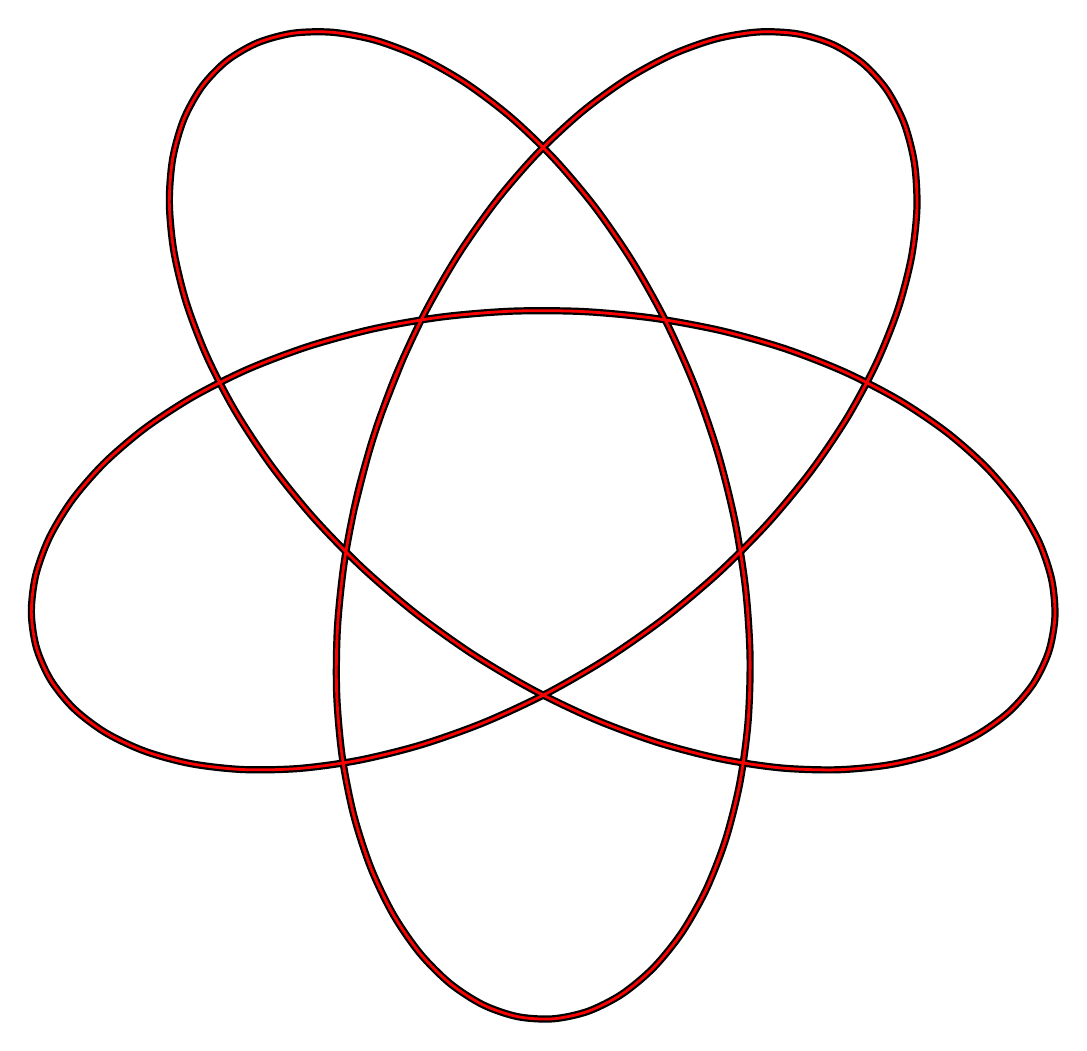
\begin{tikzpicture}[rotate=-18]
     \draw[scale=.5,samples at={-6.4,-6.3,...,6.4},
                smooth,thick,
                variable=\t,
                double= red,
                double distance = 1pt]
           plot ({3*(1.5*cos(\t r) +3*cos(1.5*\t r))},%
                 {3*(1.5*sin(\t r) -3*sin(1.5*\t r))});
    \begin{scope}[rotate=36]
       \grStar[prefix=a,RA=2.2]{6}%
       \grEmptyCycle[prefix=b,RA=4.4]{5}%
    \end{scope}
    \end{tikzpicture}
  \end{tkzexample}

\end{center}

\endinput